\section{ 君がいない (B-version)}
\large{

\ruby{君}{きみ}がいない

あの\ruby{頃}{ころ}の\ruby{二人}{ふたり}も \ruby{今}{いま}はいない
\\

\ruby{本当}{ほんとう}は \ruby{少}{すこ}しだけ\ruby{悔}{く}やんでるわ

\ruby{何故}{なぜ}なの? \ruby{君}{きみ}に\ruby{出会}{であ}い fall in love

\ruby{無口}{むぐち}でも そんなとこ\ruby{好}{す}きだったのに

\ruby{君}{き}が\ruby{嘘}{うそ}をつくなんてね

ときめきが やすらぎに\ruby{変}{か}われば

\ruby{刺激}{しげき}という \ruby{スパイス}{spice}だって\ruby{必要}{ひつよう}かもね
\\

\ruby{君}{きみ}がいない

やさしかった\ruby{君}{きみ} \ruby{今}{いま}はいない
\\

\parpic[r]{
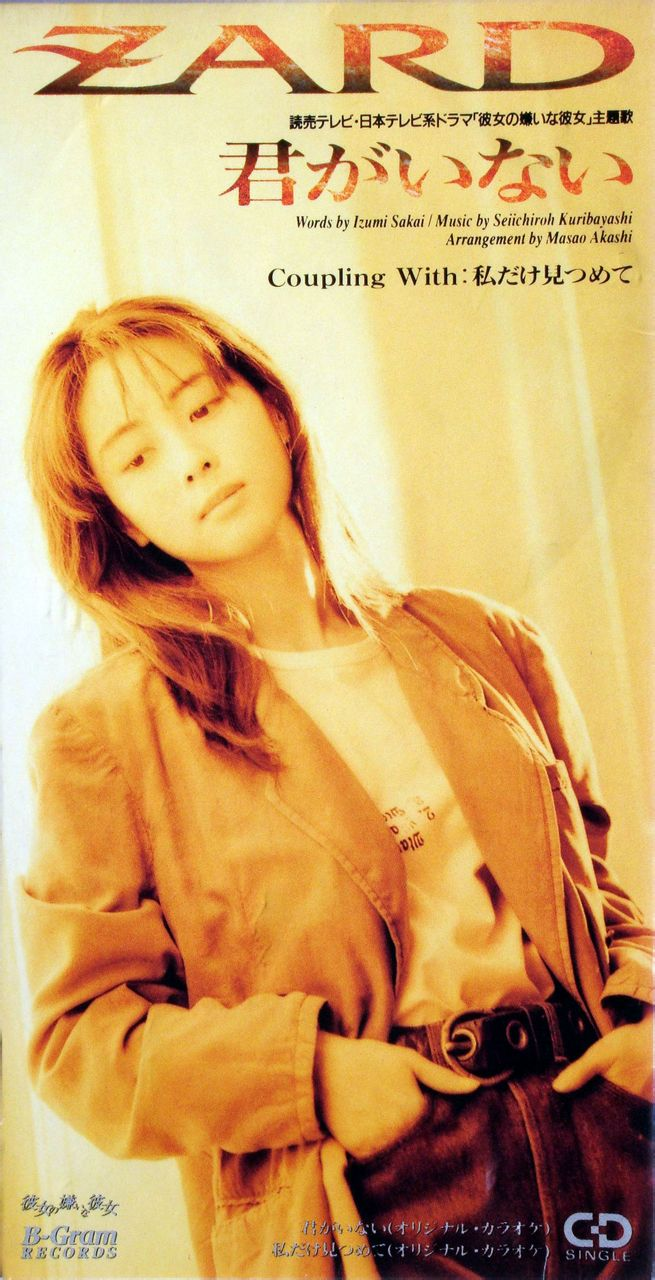
\includegraphics[width=0.3\textwidth]{S7.jpg}}

よく\ruby{行}{い}った \ruby{海岸}{かいがん}\ruby{沿}{ぞ}いの\ruby{店}{みせ}を

\ruby{通}{とお}るたび \ruby{少}{すこ}し\ruby{胸}{むね}が\ruby{痛}{いた}い

\ruby{逃}{に}げてゆく\ruby{幸}{しあわ}せに\ruby{気}{き}づいた\ruby{時}{とき}

\ruby{人}{ひと}は“もう\ruby{戻}{もど}れない”と\ruby{思}{おも}うの

やりきれない\ruby{週末}{しゅうまつ}の\ruby{メニュー}{menu}は

\ruby{思}{おも}い\ruby{出}{で}を\ruby{整理}{かたづけ}たり \ruby{映画}{えいが}を\ruby{見}{み}たり
\\

\ruby{君}{きみ}がいない

あの\ruby{頃}{ころ}の\ruby{二人}{ふたり}も \ruby{今}{いま}はいない

\ruby{何}{なに}もかも \ruby{時間}{とき}のすれ\ruby{違}{ちが}いと

\ruby{感}{かん}じた その\ruby{時}{とき} \ruby{切}{せつ}なく good-bye
\\

\ruby{君}{きみ}がいない

あの\ruby{頃}{ころ}の\ruby{二人}{ふたり}も \ruby{今}{いま}はいない

\ruby{何}{なに}もかも \ruby{時間}{とき}のすれ\ruby{違}{ちが}いと

\ruby{感}{かん}じた その\ruby{時}{とき} \ruby{切}{せつ}なく good-bye

}